\documentclass[11pt]{article}
\pdfpxdimen=1in
\divide\pdfpxdimen by 300
 
\usepackage[latin1]{inputenc}
\usepackage[T1]{fontenc}
\usepackage[english]{babel}
\usepackage{mathtools, bm}
\usepackage{amssymb, bm}
\usepackage{float}

\usepackage{caption} % to center captions
\usepackage{subcaption} % subcaption for figures side by side

\usepackage{booktabs} % for super cool table
\usepackage[table,xcdraw]{xcolor}  % to put color in tables
\usepackage{tcolorbox} % add box
\usepackage{commath} % for absolute values

\usepackage[parfill]{parskip}
\usepackage{graphicx}
\usepackage{hyperref}
\usepackage[top=0.8in, bottom=0.8in, left=1in, right=1in]{geometry}
\usepackage{listings}
\usepackage{multirow}


\renewcommand\thesubsection{\thesection.\arabic{subsection}} % Subsection starting with A, B, ...

\renewcommand\thefigure{\thesubsection.\arabic{figure}}

\newcommand{\horrule}[1]{\rule{\linewidth}{#1}} % Create horizontal rule command with 1 argument of height

\numberwithin{figure}{section} % to have per-section figure numbering

\title{	
\normalfont \normalsize 
\textsc{Master MVA \\
Reinforcement Learning} \\ [20pt]
\horrule{0.5pt} \\[0.2cm] % Thin top horizontal rule
\textbf{TP 3}: Reinforcement Learning With Function Approximation \\
\horrule{2pt} \\[0.3cm] % Thick bottom horizontal rule
}

\author{Victor Busa \\
   \texttt{victor.busa@ens-paris-saclay.fr}}

\date{\normalsize\today}

\begin{document}

\maketitle

\section{On-Policy Reinforcement Learning with Parametric Policy}
\subsection{Question 1}
See Python code for the implementation of the \emph{REINFORCE} algorithm for the linear-quadratic Gaussian regulation (LQG) problem. For this problem $\theta^* = -0.59$. I used the following parameters to run the experiments:

\begin{itemize}
\item $N = 100$: number of episodes to collect
\item $T = 100$: each trajectory have at most T time steps
\item $n\_itr = 100$: number of policy parameters update
\item $\gamma = 0.9$: discount factor
\item $n\_runs = 5$: number of times we run the algorithm to get an average
\end{itemize}

\subsubsection{Constant Step}
For the constant step, I've tuned the learning rate $\alpha$ parameter. Figures~\ref{fig:cst_avg_reward} and~\ref{fig:cst_mean_param} show the value of the average reward $R$ and the $\widehat{\theta}$ parameter for different values of $\alpha$:

\begin{figure}[H]
		\centering
		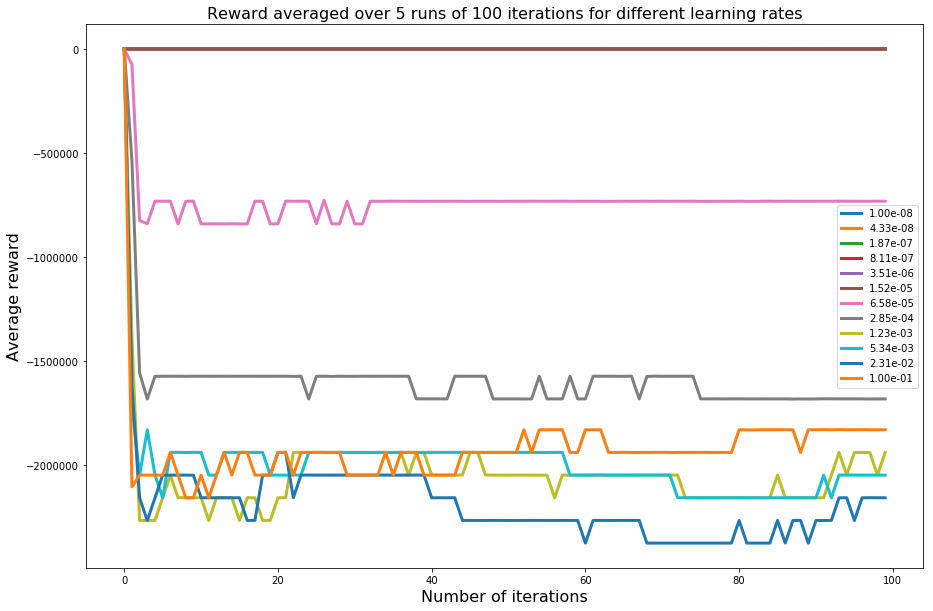
\includegraphics[width=0.9\linewidth]{images/avg_reward}
		\caption{average reward over 5 runs of 100 iterations each for different values of the learning rate $\alpha$}
		\label{fig:cst_avg_reward}
\end{figure}

\begin{figure}[H]
		\centering
		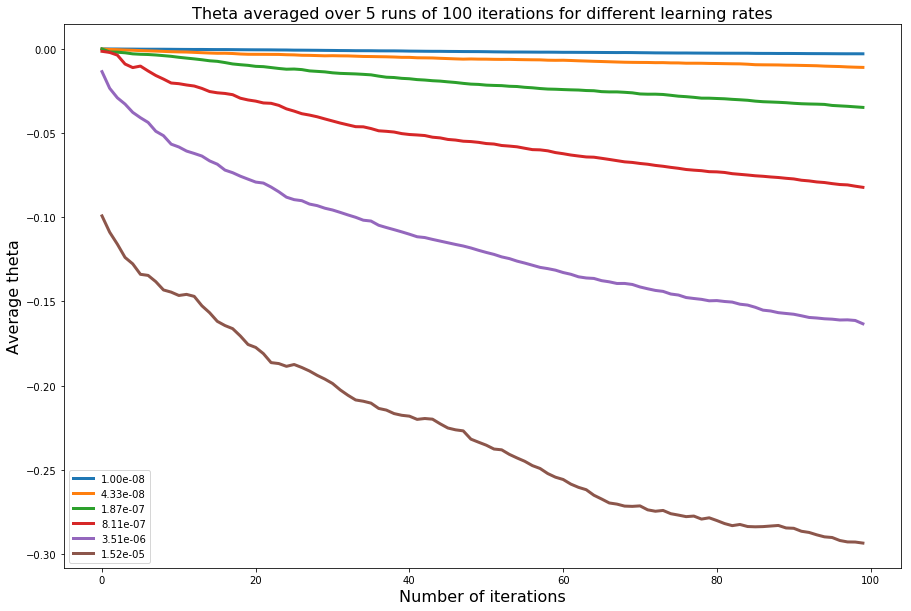
\includegraphics[width=0.9\linewidth]{images/avg_theta_consistent}
		\caption{average parameter $\widehat{\theta}$ over 5 runs of 100 iterations each for different values of the learning rate $\alpha$}
		\label{fig:cst_mean_param}
\end{figure}

According to the Figures we can see that the best value of $\alpha$ is $\alpha$ = 1.52e-5 as $\widehat{\theta}$ converges faster towards $\theta^* = -0.59$. We will use this value of $\alpha$ and we will tune the learning decay in the next section.

\subsubsection{Annealing Step}
Using the best value of $\alpha$ ($\alpha$ = 1.52e-5) found for the constant step, we will tune the learning decay. Figures~\ref{fig:ann_avg_reward} and~\ref{fig:ann_mean_param} show the value of the average reward $R$ and the $\widehat{\theta}$ parameter for different values of the learning decays:

\begin{figure}[H]
		\centering
		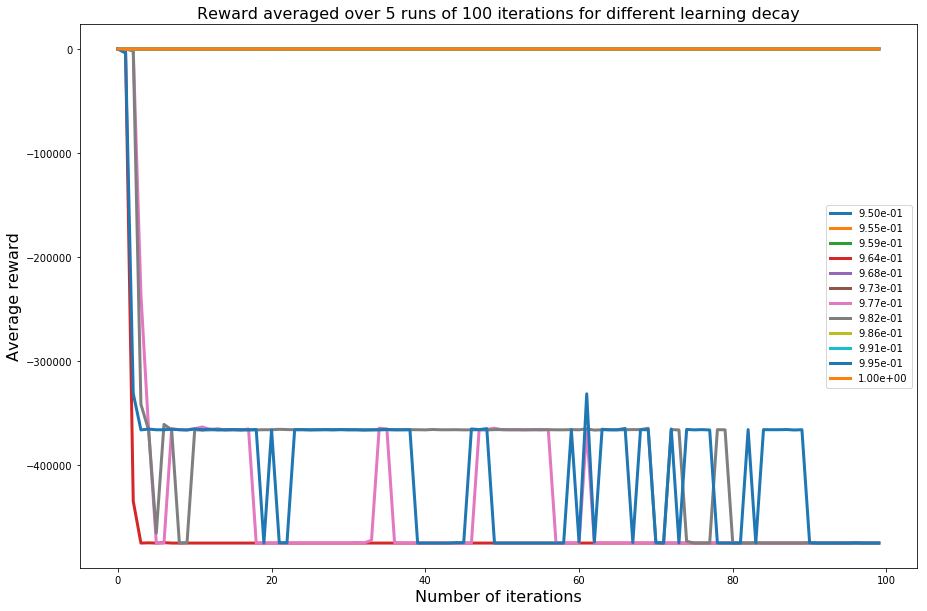
\includegraphics[width=0.9\linewidth]{images/ld_avg_reward}
		\caption{average reward over 5 runs of 100 iterations each for different values of the learning decays}
		\label{fig:ann_avg_reward}
\end{figure}

\begin{figure}[H]
		\centering
		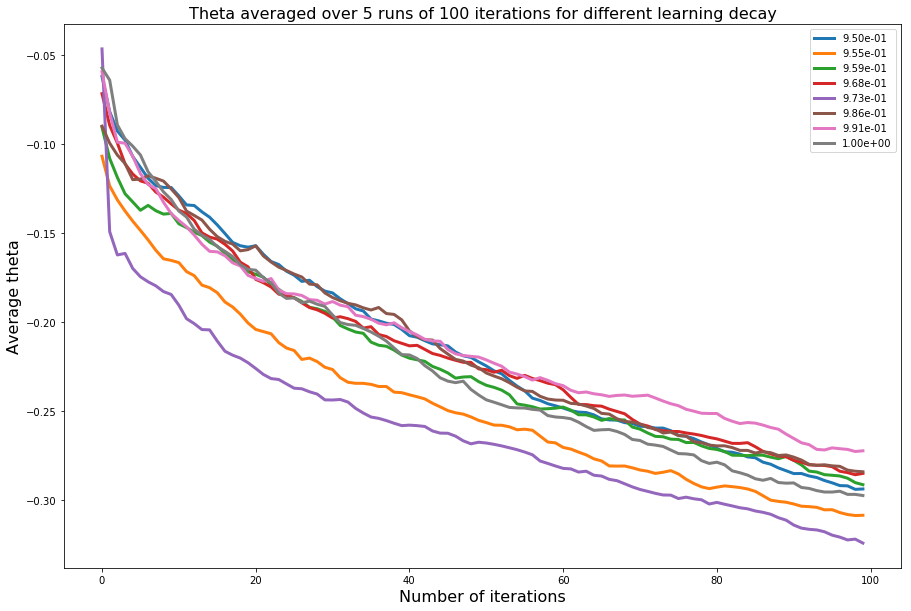
\includegraphics[width=0.9\linewidth]{images/ld_theta_consistent}
		\caption{average parameter $\widehat{\theta}$ over 5 runs of 100 iterations each for different values of the learning decays}
		\label{fig:ann_mean_param}
\end{figure}

According to Figures~\ref{fig:ann_avg_reward} and~\ref{fig:ann_mean_param}, the best learning decay for this experiment is $0.973$. \\
\textbf{Note}: In practice it is very difficult to tune both the learning rate and the learning decay and here I chose to tune the learning decay only for a fixed value of the learning rate. What we should instead do is: use a high learning rate $\alpha$ at the beginning of the experiment and a high learning decay. Then decrease the learning rate by the learning decay and decrease the learning decay at each iterations. What should be even better is not to decrease the learning decay at each iteration but instead decrease it when the norm of two successive update of the parameters $\theta$ is below a certain threshold. I don't have the time to run these experiments as the algorithm takes some times to terminate.

\subsubsection{Adam Step}
In this experiment I used the adam optimizer and I've tuned the learning rate $\alpha$for a fixed value of $\beta_1 = 0.9$, $\beta_2 = 0.999$, $\epsilon = 10^{-8}$. Here I've chosen to test the REINFORCE algorithm for 12 values of $\alpha$ logarithmically spaced in $[10^{-3}, 10^{-1}]$. Figures~\ref{fig:adam_avg_reward} and~\ref{fig:adam_mean_param} show the value of the average reward $R$ and the $\widehat{\theta}$ parameter for different values of the learning rates.

\textbf{Note}: I've deleted inconsistent values of the learning rates $\alpha$ before plotting the graphs, that is why there is no $12$ different values of $\alpha$.

\begin{figure}[H]
		\centering
		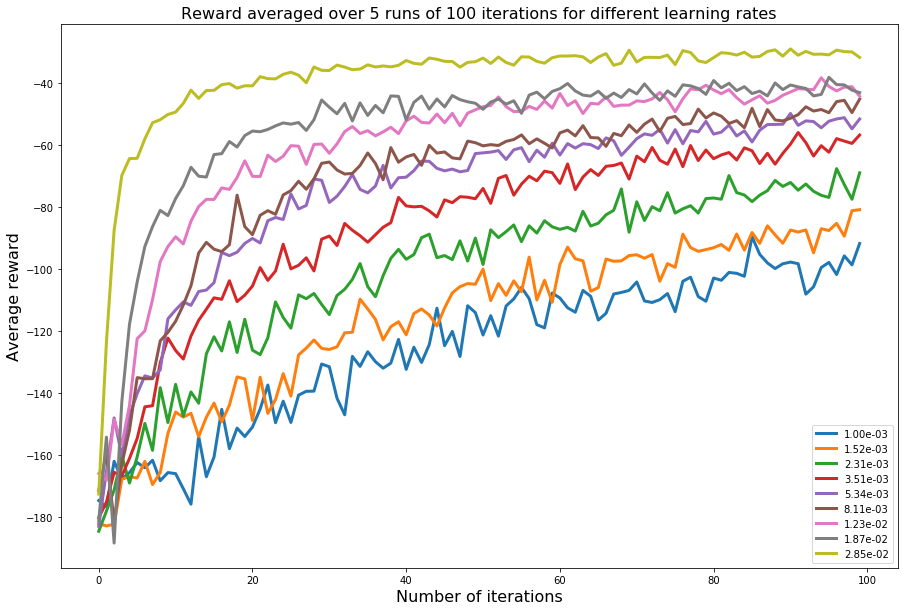
\includegraphics[width=0.9\linewidth]{images/adam_avg_reward}
		\caption{average reward over 5 runs of 100 iterations each for different values of the learning rates}
		\label{fig:adam_avg_reward}
\end{figure}

\begin{figure}[H]
		\centering
		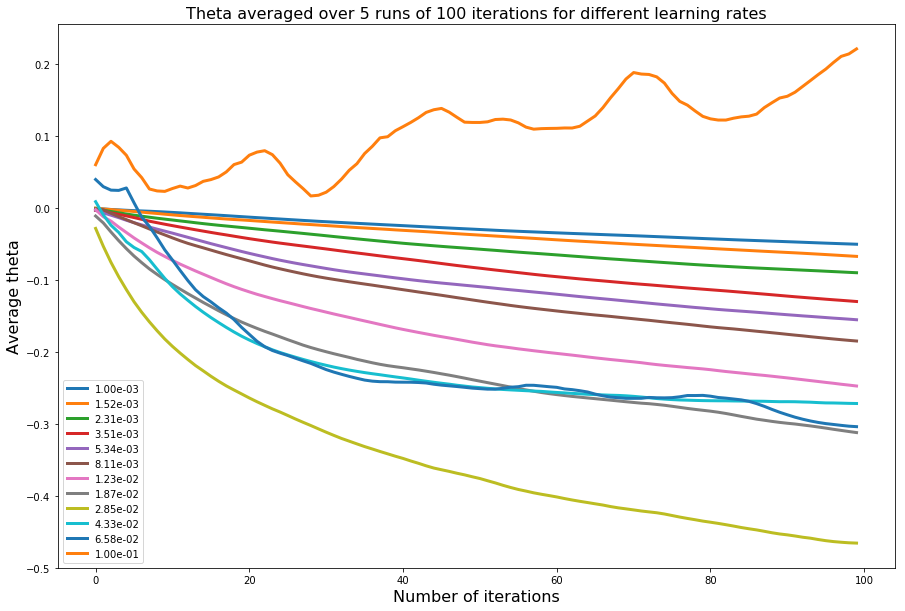
\includegraphics[width=0.9\linewidth]{images/adam_avg_theta_consistent}
		\caption{average parameter $\widehat{\theta}$ over 5 runs of 100 iterations each for different values of the learning rates}
		\label{fig:adam_mean_param}
\end{figure}

According to Figures~\ref{fig:adam_avg_reward} ~\ref{fig:adam_mean_param} the best value for $\alpha$ is $\alpha$ = 2.85e-2.

\subsection{Conclusion}
$\alpha_t$ is the learning rate parameter. A high value of $\alpha_t$ will make a big step in the direction of the gradient of the function we computed and hence. Yet, if the step is too big, in the next iteration it might result in a value of the function we tried to minimize which is higher then at the previous iteration. On the contrary, if the value of $\alpha_t$ is too low, the value will likely decrease at each iteration but it won't decrease a lot and the algorithm will take lots of time to converge. Hence it is very important to tune this parameter. Adam optimizer is a gradient descent method that takes into account the moment or velocity of previous iteration in order to accelerate the convergence of the next iteration. \\
$N$ (the number of trajectories generated) matters in the sense that the more trajectories we collect the more accurately the algorithm will converge at each iteration. Indeed $N=1$ is synonym of a stochastic gradient descent and thus the algorithm run faster but will converge more slowly (and the convergence curve will have a serrated shape).

\subsection{Question 2: Trying different values of N: number of trajectories}
As discussed shortly in the Conclusion part, the lowest the value of N is, the fastest\footnote{in term of computational time} the algorithm will run. Yet, the algorithm will converge more slowly as the direction of the gradient for few trajectories isn't representative enough of the true direction to consider to minimize the gradient. The higher the value of N is the more accurately the algorithm will converge to the true direction that minimize the gradient but it will also takes more time at each iteration due to the high number of trajectories to consider at each iteration. Figures~\ref{fig:q2_reward} and ~\ref{fig:q2_theta} show the value of the average return and the average theta for 5 distinct runs and different values $N$.

\begin{figure}[H]
		\centering
		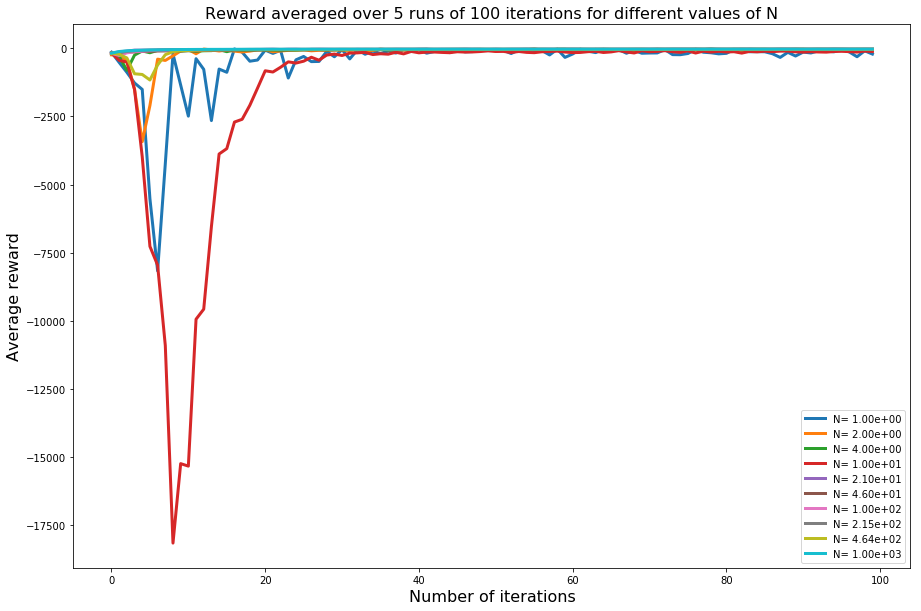
\includegraphics[width=0.8\linewidth]{images/q2_reward}
		\caption{average return $J(\pi_k)$ in function of the number of iterations $k$ obtained by the fitted-Q iteration algorithm applied to the LQG problem for different values of $N$ (the number of trajectories considered)}
		\label{fig:q2_reward}
\end{figure}

\begin{figure}[H]
		\centering
		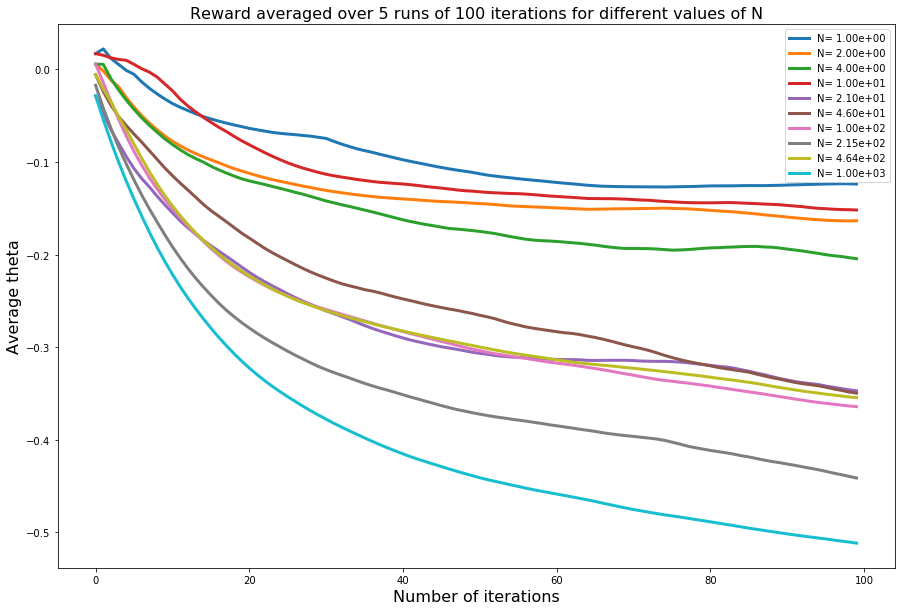
\includegraphics[width=0.8\linewidth]{images/q2_theta}
		\caption{average theta $\widehat{\theta}$ in function of the number of iterations $k$ obtained by the fitted-Q iteration algorithm applied to the LQG problem for different values of $N$ (the number of trajectories considered)}
		\label{fig:q2_theta}
\end{figure}

Naturally we can see that high value of $N$ allow the algorithm to converge more quickly to the true value $\theta^*$ will it also takes more time to compute (6 min on my compute\footnote{See code}). On the other hand lower values of $N$ converge slowly much takes less time to compute. Hence we have to choose $N$ carefully to balance between computational time and convergence velocity. $N \approx 200$ seems to be a good pragmatical choice.

\section{On-Policy Reinforcement Learning with Parametric Policy}
\subsection{Implementation}
See Python code for the implementation of the algorithm. I chose to stop the algorithm either went it attains a number of maximum iterations (set by default to 100) or when $\ell_2(\theta_k - \theta_{k-1}) < \epsilon$ with $\epsilon=10^{-12}$ by default.

\subsection{Experimentation}
Using a discount parameter $\gamma = 0.9$ and a value of $\lambda$ (the regularization parameter) of 2, the linear fitted Q iteration algorithm performs well and converges in one iteration. The Figure~\ref{fig:fqi} shows the average reward obtained from running the fitted-Q iteration algorithm on the linear-quadratic Gaussian regulation (LQG) problem in function of the number of iterations $k$.

\begin{figure}[H]
		\centering
		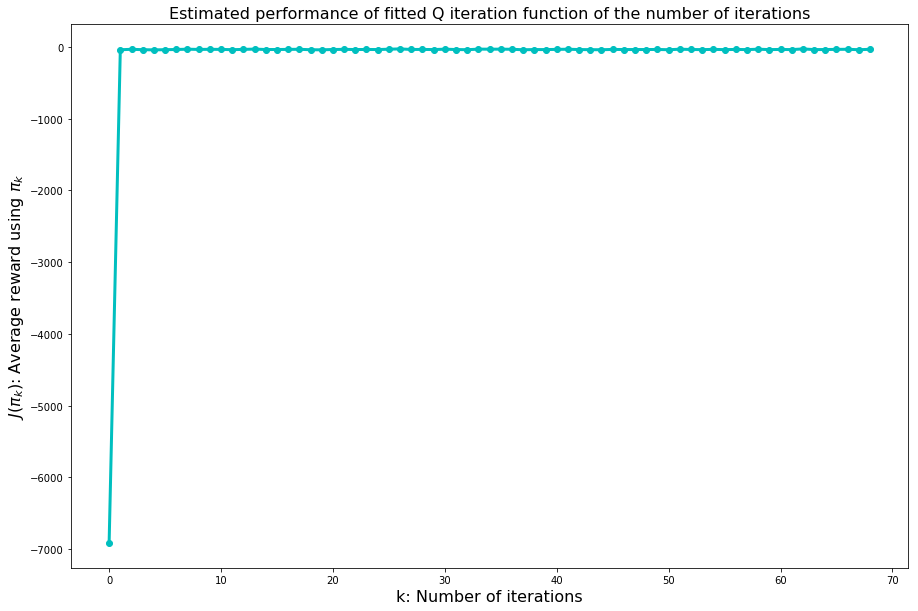
\includegraphics[width=0.9\linewidth]{images/fqi_single}
		\caption{average return $J(\pi_k)$ in function of the number of iterations $k$ obtained by the fitted-Q iteration algorithm applied to the LQG problem}
		\label{fig:fqi}
\end{figure}


\textbf{Note}: I've played with the parameters $\alpha$ and $\gamma$ to see if it impacts the performance of the algorithm for the LQG problem. Apparently it hasn't much influence on the performance. Graphs ~\ref{fig:fqi_alpha} and \ref{fig:fqi_gamma} that show the result of the fitted Q iteration in function of $\alpha$ or $\gamma$ are displayed below.

\begin{figure}[H]
		\centering
		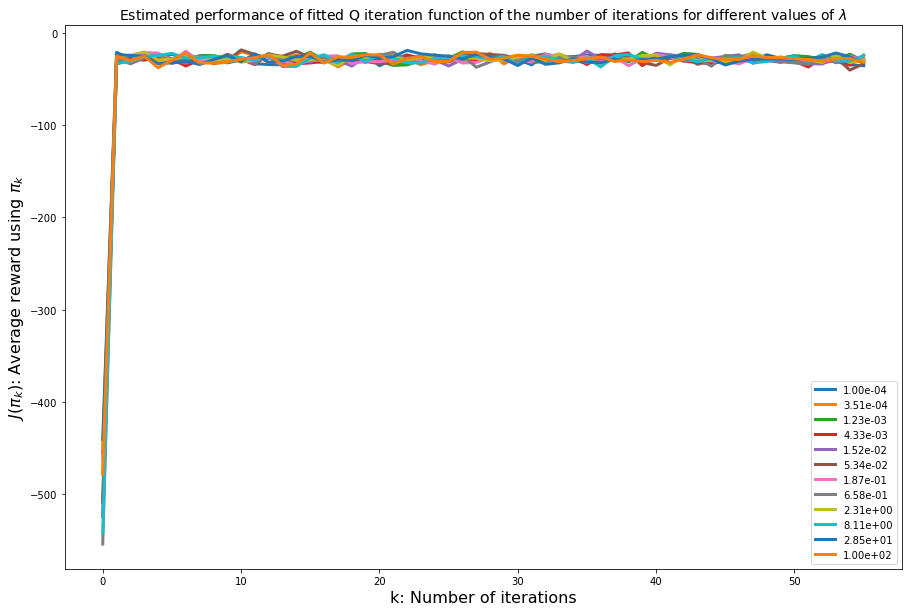
\includegraphics[width=0.9\linewidth]{images/fqi_alpha}
		\caption{average return $J(\pi_k)$ in function of the number of iterations $k$ obtained by the fitted-Q iteration algorithm applied to the LQG problem for different values of $\alpha$}
		\label{fig:fqi_alpha}
\end{figure}

\begin{figure}[H]
		\centering
		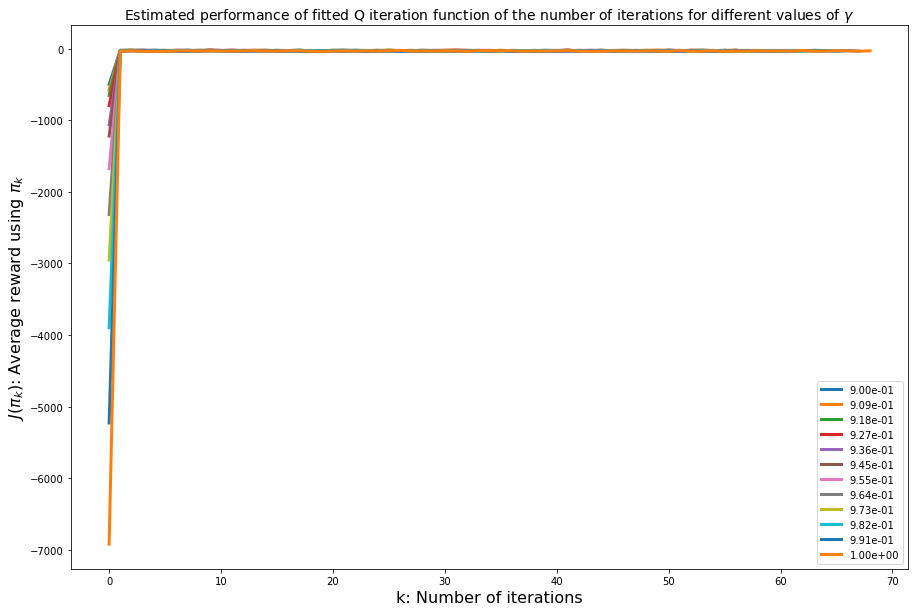
\includegraphics[width=0.9\linewidth]{images/fqi_gamma}
		\caption{average return $J(\pi_k)$ in function of the number of iterations $k$ obtained by the fitted-Q iteration algorithm applied to the LQG problem for different values of $\gamma$}
		\label{fig:fqi_gamma}
\end{figure}


\end{document}